\section{Introduction}

Recent progress in large language models (LLMs) has shifted from scaling model size or pretraining data to improving inference-time behavior, a direction known as \textit{test-time scaling}\cite{snell2024scalingllmtesttimecompute,muennighoff2025s1simpletesttimescaling}. Test-time scaling is designed to enhance model performance by allocating additional computation during inference without modifying the model's parameters. This includes techniques such as Chain-of-Thought~\cite{cot}, Tree-of-Thought~\cite{tot}, and others~\cite{touvron2023llama2openfoundation,self_cot,least_cot,press2023measuring,graph_of_thought}. These approaches promote more deliberate and interpretable \emph{reasoning} within the LLM, enabling it not only to recognize patterns but also to derive conclusions, generate explanations, and solve tasks that require step-by-step logic.

\begin{figure}[t]
    \centering
    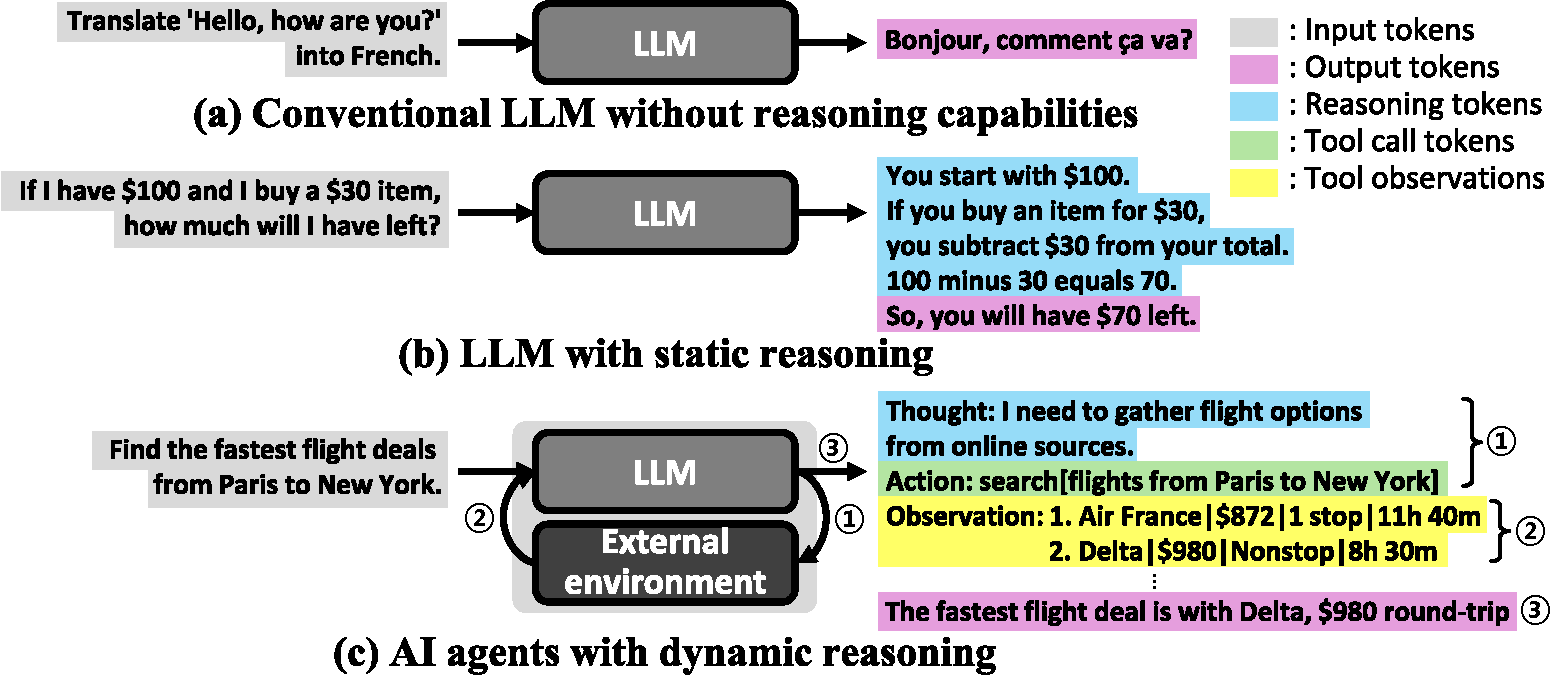
\includegraphics[width=0.485\textwidth]{./fig/intro_overview}
    % \vspace{-1.8em}
    \caption{
    Overview of reasoning strategies in LLM-based systems.
    (a) Conventional LLMs map inputs directly to outputs in a single forward pass, with no explicit intermediate reasoning.
    (b) Reasoning‑enhanced LLMs internally create intermediate steps (e.g., sampling alternative responses or extending token sequences) to deepen or diversify their thought process.
    (c) AI agents augment this reasoning by
    \wcirclednum{1} planning and invoking external tools, \wcirclednum{2} observing the outcomes and adapting their internal reasoning, and iteratively refining their decision-making until they \wcirclednum{3} generate the final answer.
    }
    \label{fig:intro_overview}
    \vspace{-0.6em}    
\end{figure}

Deploying these reasoning-enhanced LLMs, however, comes at an immense computational cost. Even in current \textbf{static reasoning} models which follow fixed input-output mappings without external tool interaction (\fig{fig:intro_overview}(a,b)), LLMs run on thousands of GPUs, whose power, cooling, and capital costs drive monthly expenses into the tens of millions of dollars~\cite{openai_cost_2023}. A single ChatGPT query is estimated to consume about ten times the electricity of a typical web search~\cite{AI_energy_footprint} and requires a substantial amount of cooling water~\cite{AI_water_footprint}. As a result, hyperscalers are investing at an unprecedented scale. Meta has already committed over \$10 billion to AI infrastructure~\cite{meta_10_billion}, and Microsoft operates custom AI supercomputers that draw tens to hundreds of megawatts. As an example, xAI’s Colossus AI supercomputer alone employs approximately 100,000 Nvidia H100 GPUs, consuming 150 megawatts in total, with the GPUs alone accounting for around 70 megawatts~\cite{xAI_collosus}. For perspective, traditional hyperscale data centers typically draw between 10 and 100 megawatts~\cite{hyperscale_datacenter}, while advanced semiconductor fabs, such as those operated by Samsung and TSMC, consume several hundred megawatts each~\cite{tsmc_fab_power,fab_power}. Analysts forecast that total AI infrastructure spending will surpass \$1 trillion within this decade~\cite{capex_forecast}, raising serious concerns about power grid sustainability and the economic viability of large-scale LLM deployment.


Given this landscape, the emergence of \emph{AI agents} powered by LLMs with \textbf{dynamic reasoning} threatens to exacerbate these already formidable infrastructure pressures dramatically. Unlike static reasoning models, dynamic reasoning represents an advanced form of test-time scaling that significantly boosts capabilities through active interaction with external environments (\fig{fig:intro_overview}(c)). Specifically, AI agents continuously plan, invoke external tools, observe outcomes, and iteratively refine their reasoning, often performing dozens of inference calls to satisfy a single user request~\cite{react,reflexion,lats}. Without substantial system-level innovations, per-request computational costs could increase by orders of magnitude, making large-scale deployment of agents economically and environmentally prohibitive. Industry leaders are already responding to these challenges: OpenAI’s planned Stargate project~\cite{openai_stargate} and Meta's next generation AI data center Hyperion~\cite{meta_hyperion_prometheus} are each projected to require multiple ``gigawatts'' of power capacity, with costs reaching hundreds of billions of dollars. Yet, despite these developments, the computer architecture community has largely focused on static LLMs, leaving the infrastructure implications of dynamic reasoning workloads underexplored.


To address this critical gap, this paper presents a rigorous, quantitative evaluation of the computational and infrastructural costs of dynamic reasoning. We systematically characterize resource utilization, latency implications, and energy demands inherent in the iterative execution patterns of AI agents.
While the serving characteristics of static reasoning LLMs are well understood within the research community, our work presents the first comprehensive, system-level characterization of agent serving costs across diverse configurations and workloads. Each component of our analysis—including the characterization of agent workflows themselves, serving performance, and the impact of test-time scaling—quantifies a distinct dimension of this cost structure, collectively building a unified understanding of its infrastructure-level implications.
Our analysis highlights the critical system-level challenges faced when deploying AI agents and identifies opportunities for optimization through architectural improvements, enhanced inference algorithms, and intelligent resource allocation strategies. To the best of our knowledge, this work is the first to provide a system-level characterization of dynamic reasoning in AI agents, grounded in quantitative analysis of end-to-end infrastructure behavior across diverse agentic workflows\footnote{Open-sourced at \href{https://github.com/VIA-Research/AgentBench}{https://github.com/VIA-Research/AgentBench.}}. A key contribution and objective of our study is to quantitatively assess the AI infrastructure cost of dynamic reasoning deployments, and to inform and caution the research community about the urgent need for sustainable, efficient design principles to bridge the gap between advanced algorithmic capabilities and practical, scalable, and sustainable deployment.
